\documentclass[11pt,a4paper]{article}
\usepackage{amssymb,amsfonts,amsmath,calc,tikz,pgfplots,geometry}
\usepackage{color}   %May be necessary if you want to color links
\usepackage{hyperref}
\usepackage{amsthm}
\usepackage{minted}
\usepackage{listings}
\usepackage[linesnumbered,ruled,vlined]{algorithm2e}
\usetikzlibrary{positioning}
\geometry{margin=1in}
\hypersetup{
    colorlinks=false, %set true if you want colored links
    linktoc=all,   %set to all if you want both sections and subsections linked
    linkcolor=black,  %choose some color if you want links to stand out
}
%%%%%%%%%%%%%%%%%%%%%%%%%%%%%%%%%%%%%%%%%%%%%%%%%%%%%%%%%%%%%%%%%%%%%%%%%%%%%%%
\theoremstyle{plain}
\newtheorem{theorem}{Theorem}[section]
\newtheorem{lemma}[theorem]{Lemma}
\newtheorem{proposition}[theorem]{Proposition}
\newtheorem{corollary}[theorem]{Corollary}
\newtheorem{definition}{Definition}[section]
\newtheorem{remark}{Remark}[section]
\DeclareMathOperator{\lcm}{lcm}
\newcommand{\N}{\mathbb{N}}
\newcommand{\Z}{\mathbb{Z}}
\newcommand{\Q}{\mathbb{Q}}
\newcommand{\R}{\mathbb{R}}
\newcommand{\C}{\mathbb{C}}
\newcommand{\F}{\mathbb{F}}
\newcommand{\Omicron}{O}
\newcommand{\ip}[2]{\langle #1, #2 \rangle}
\newcommand{\bigslant}[2]
{{\raisebox{.2em}{$#1$}\left/\raisebox{-.2em}{$#2$}\right.}}
%%%%%%%%%%%%%%%%%%%%%%%%%%%%%%%%%%%%%%%%%%%%%%%%%%%%%%%%%%%%%%%%%%%%%%%%%%%%%%%
\title{\textbf{Algorithms}}
\author{Yeheli Fomberg}
\date{326269651}
\usepackage{amsmath}
\begin{document}
	\maketitle
	\newpage
	\section{Preliminaries}
	This is a course about algorithms, and since many problems we are going to
	solve will require some knowledge about graphes we will write here
	some basic definitions so that we always have a reference if we forget
	something.
	\begin{definition}
	An ordered pair $G=(V,E)$ of $V$ a set of vertices, and $E$ a 
	of $V \times V$ - a set of unordered pairs of vertices or ``edges'' is 
	called a \textbf{graph}.
	\end{definition}
	We can imagine graphes as nodes with names or values that represent them
	and the edges connect the nodes. For example we can consider the following
	graph $G=(\{1,2,3\}, \{(2,3),(3,1)\})$
	\begin{center}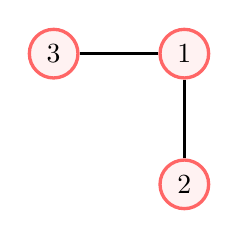
\begin{tikzpicture}[
	nstyle/.style={circle, fill=red!5, draw=red!60, very thick, 
	minimum size=5mm,}
	]
	\node[nstyle] (1) {$1$};
	\node[nstyle] (2) [below=of 1] {$2$};
	\node[nstyle] (3) [left=of 1] {$3$};
	
	\draw[very thick] (1.south) to (2.north);
	\draw[very thick] (3.east) to (1.west);
	\end{tikzpicture}\end{center}
	It looks very nice, we can think of it also as relations between people
	just by changing the names of the vertices:
	\begin{center}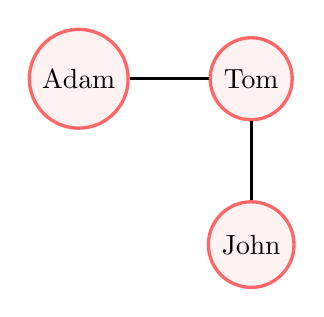
\begin{tikzpicture}[
	nstyle/.style={circle, fill=red!5, draw=red!60, very thick, 
	minimum size=5mm,}
	]
	\node[nstyle] (1) {Tom};
	\node[nstyle] (2) [below=of 1] {John};
	\node[nstyle] (3) [left=of 1] {Adam};
	
	\draw[very thick] (1.south) to (2.north);
	\draw[very thick] (3.east) to (1.west);
	\end{tikzpicture}\end{center}
	This graph may represent that Adam knows Tom and John knows Adam but
	Adam and John don't know each other. We may also consider the relation
	of $A$ loves $B$. In this case we need to define a new kind of graph,
	since even if Adam loves Tom, that doesn't mean that Tom loves Adam.
	\begin{definition}
	An ordered pair $G=(V,E)$ of $V$ a set of vertices, and $E$ a subset
	of $V \times V$ - a set of ordered pairs of vertices is
	called a \textbf{dircted graph}.
	\end{definition}
	One such example coud be:
	\begin{center}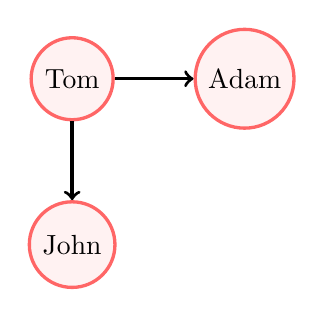
\begin{tikzpicture}[
	nstyle/.style={circle, fill=red!5, draw=red!60, very thick, 
	minimum size=5mm,}
	]
	\node[nstyle] (1) {Tom};
	\node[nstyle] (2) [below=of 1] {John};
	\node[nstyle] (3) [right=of 1] {Adam};
	
	\draw[->,very thick] (1.south) to (2.north);
	\draw[<-,very thick] (3.west) to (1.east);
	\end{tikzpicture}\end{center}
	Oh no! Tom loves two people, yet he isn't loved by anyone :( \\
	Notice how changing the placement of the vertices doesn't change the 
	graph itself.
	
	\newpage
	\begin{definition}
	A \textbf{walk} is a finite or infinite sequence of edges which 
	joins a sequence of vertices.
	\end{definition}
	\begin{definition}
	A \textbf{trail} is a walk in which all edges are distinct.
	\end{definition}
	\begin{definition}
	A \textbf{path} is a trail in which all vertices 
	(and therefore also all edges) are distinct.
	\end{definition}
	\begin{definition}
	A \textbf{simple graph} is a graph in which there are no edges from
	a vertex to itself, or multiple edges from on vertex to another.
	\end{definition}
	For example the following is not a simple graph:
	\begin{center}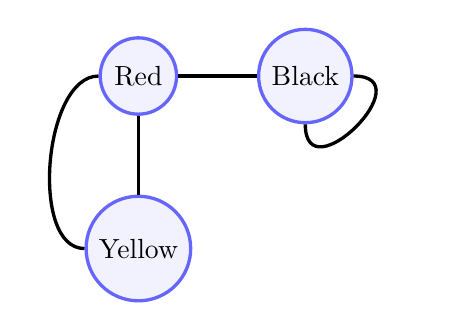
\begin{tikzpicture}[
	nstyle/.style={circle, fill=red!5, draw=red!60, very thick, 
	minimum size=5mm,}
	]
	\node[nstyle, fill=blue!5, draw=blue!60] (1) {Red};
	\node[nstyle, fill=blue!5, draw=blue!60] (2) [below=of 1] {Yellow};
	\node[nstyle, fill=blue!5, draw=blue!60] (3) [right=of 1] {Black};
	
	\draw[very thick] (1.south) to (2.north);
	\draw[very thick] 
	(1.west) .. controls +(left:7mm) and +(left:7mm) .. (2.west);
	\draw[very thick] (3.west) to (1.east);
	\draw[very thick] 
	(3.east) .. controls +(right:9mm) and +(down:9mm) .. (3.south);
	\end{tikzpicture}\end{center}
	\begin{definition}
	A \textbf{circuit} is a non-empty trail in which the first and last 
	vertices are equal (closed trail).
	\end{definition}
	\begin{definition}
	A \textbf{cycle} or \textbf{simple circuit} is a circuit in which only 
	the first and last vertices are equal.
	\end{definition}
	For example in the graph below:
	\begin{center}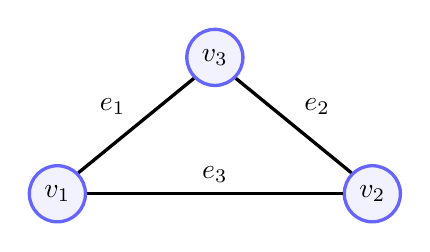
\begin{tikzpicture}[
	nstyle/.style={circle, fill=red!5, draw=red!60, very thick, 
	minimum size=5mm,}
	]
	\draw(-1,0)node[nstyle, fill=blue!5, draw=blue!60] (red) {$v_1$};
	\draw(3,0)node[nstyle, fill=blue!5, draw=blue!60] (yellow) {$v_2$};
	\draw(60:2)node[nstyle, fill=blue!5, draw=blue!60] (black) {$v_3$};
	\draw[very thick] (black.south west) to 
	node[above left] {$e_1$}
	(red.north east);
	\draw[very thick] (black.south east) to 
	node[above right] {$e_2$}
	(yellow.north west);
	\draw[very thick] (red.east) to 
	node[above] {$e_3$}
	(yellow.west);
	\end{tikzpicture}\end{center}
	We have the cycle $C = (v_1,e_1,v_3,e_2,v_2,e_3,v_1)$.
	\begin{definition}
	The \textbf{distance} between two vertices $u$, $v$ is denoted as 
	$\delta(u,v)$ and is the length of a shortest directed path from 
	$u$ to $v$ consisting of arcs, provided at least one such path exists.
	\end{definition}
	
	
	\newpage
	
	\newpage
	\section{BFS}
	The BFS (Breadth First Search) algorithm is an algorithm that travereses
	all the vertices in the graph in a way breadth first approach, meaning
	that if we start at vertex $s$ we will not traverse vertices in distance
	$i$ from $s$ before visiting all vertices of distance $<i$ from $s$.
	We can also use this algorithm to efficiently find the distance of
	any vertex from $s$. 
	Suppose we need to find the distance between the points $s$, $v$ on a 
	graph $G=(V,E)$,  we could first look at $u$, then consider all of its 
	neighbors and mark their distance from $u$ as $1$ and then consider all 
	of the neighbors unvisited neighbors and mark their distance from $u$ as 
	$2$ and so on. The reason this is called ``Breadth First Search'' is 
	because we are going to mark
	all vertices with distacne $i$ from $u$ before giving the vertices
	and distance $i+1$ from $u$. What I just described is how to algorithm
	is supposed to work, but we need to be more exact and write psuedo-code
	for it, then prove its correctness, and calculate its complexity.
	\begin{algorithm}
	\caption{BFS Algorithm}
	\KwIn{Graph $G=(V, E)$, starting vertex $s$}
	\KwOut{Visited vertices in BFS order}
	Initialize queue $Q$\;
	Mark all vertices as unvisited\;
	Mark the source vertex $s$ as visited and enqueue $s$ to $Q$\;
	\While{$Q$ is not empty}{
		Dequeue a vertex $v$ from $Q$\;
		\For{each neighbor $u$ of $v$}{
		    \If{$u$ is not visited}{
		        Mark $u$ as visited\;
		        Enqueue $u$ to $Q$\;
		    }
		}
	}
	\end{algorithm} \\
	This is the basic BFS algorithm that just traverses the graph. If we
	want to also find the distances of all the vertices from $s$ we can
	first initialize our approximaition distance function and correct
	it along the way.
	\begin{algorithm}
	\caption{BFS Algorithm for finding distances}
	\KwIn{Graph $G=(V, E)$, starting vertex $s$}
	\KwOut{$\lambda$ such that $\lambda = \delta$}
	Initialize queue $Q$\;
	Initialize the $\lambda(s,v)=\infty$ for every $v\in V$\;
	Redefine $\lambda(s,s)=0$ and enqueue $s$ to $Q$\;
	\While{$Q$ is not empty}{
		Dequeue the top vertex $v$ from $Q$\;
		\For{each neighbor $u$ of $v$}{
		    \If{$\lambda(s,u) = \infty$}{
		        $\lambda(s,u) = \lambda(s,v) + 1$\;
		        Enqueue $u$ to $Q$\;
		    }
		}
	}
	\end{algorithm} \\
	
	\newpage
	
	
	We need to show find its complexity and show correctness.
	First we can find the complexity. We know that in the initizlization
	we go over all the vertices so the complexity there is $O(|V|)$, and
	then every iteration we do in $O(\deg(u))$ so the total complexity
	is:
	\[
		O(|V|) + \sum_{u\in V}{O(\deg(u))} = O(|V|) + O(|E|) = O(|V|+|E|)
	\]
	To prove correctness we will show that $\delta(s,v) \le \lambda(s,v)$ and 
	$\lambda(s,v) \le \delta(s,v)$. If we have $\delta(s,v)=\infty$ then
	the inequality is correct, otherwise we can show that by induction 
	over the order the vertices enter the queue.\\
	\underline{Base case} \\
	if $v$ is the first vertex to enter the queue then we have $v=s$
	and then:
	\[
		\delta(s,s) = \lambda(s,s) = 0
	\]
	\underline{Step} \\
	Now suppose we know that for all the previous vertices that entered
	the queue we have the inequlity, by the algorithm definition we get:
	\[
		\lambda(s,v) = \lambda(s,u) + 1 \underbrace{\geq}_{\text{induction}} 
		\delta(s,v) + 1 \geq \delta(s,v)
	\]
	Which means that for all $v\in V$ we have $\delta(s,v) \le \lambda(s,v)$
	which completes one side of the proof. Try proving the other side
	yourself.
	
	\newpage
	
	\section{Topological Sorting}
	To talk about Topological sorting we first have to recall how we can 
	define simple graphes. We can define graphes using an adjacency matrix
	such that:
	\begin{enumerate}
	\item $(A)_{ij}$ will be $1$ if $(i,j)\in E$
	\item $(A)_{ij}$ will be $0$ if $(i,j)\notin E$
	\end{enumerate}
	For example the adjacency matrix for the graph:
	\begin{center}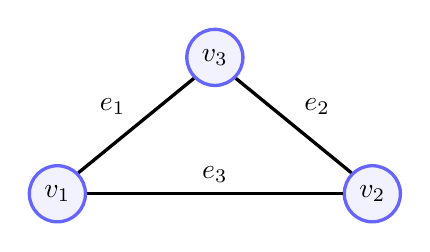
\begin{tikzpicture}[
	nstyle/.style={circle, fill=red!5, draw=red!60, very thick, 
	minimum size=5mm,}
	]
	\draw(-1,0)node[nstyle, fill=blue!5, draw=blue!60] (red) {$v_1$};
	\draw(3,0)node[nstyle, fill=blue!5, draw=blue!60] (yellow) {$v_2$};
	\draw(60:2)node[nstyle, fill=blue!5, draw=blue!60] (black) {$v_3$};
	\draw[very thick] (black.south west) to 
	node[above left] {$e_1$}
	(red.north east);
	\draw[very thick] (black.south east) to 
	node[above right] {$e_2$}
	(yellow.north west);
	\draw[very thick] (red.east) to 
	node[above] {$e_3$}
	(yellow.west);
	\end{tikzpicture}\end{center}
	is:
	\[
		A = \begin{pmatrix}
			0 & 1 & 1\\
			1 & 0 & 1\\
			1 & 1 & 0\\
		\end{pmatrix}
	\]
	And with directed graphes we can define for $i \le j$ as such:
	\begin{enumerate}
	\item $(A)_{ij}$ will be $1$ if $(i,j)\in E$
	\item $(A)_{ji}$ will be $-1$ if $(i,j)\in E$
	\item $(A)_{ij}$ will be $0$ if $(i,j)\notin E$
	\end{enumerate}
	So for example for the graph:
	\begin{center}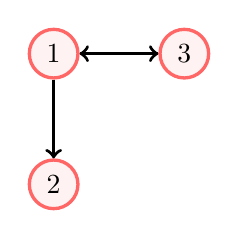
\begin{tikzpicture}[
	nstyle/.style={circle, fill=red!5, draw=red!60, very thick, 
	minimum size=5mm,}
	]
	\node[nstyle] (1) {$1$};
	\node[nstyle] (2) [below=of 1] {$2$};
	\node[nstyle] (3) [right=of 1] {$3$};
	
	\draw[->,very thick] (1.south) to (2.north);
	\draw[<-,very thick] (3.west) to (1.east);
	\draw[->,very thick] (3.west) to (1.east);
	\end{tikzpicture}\end{center}
	We get:
	\[
		A = \begin{pmatrix}
			0 & 1 & 1\\
			0 & 0 & 0\\
			-1 & 0 & 0\\
		\end{pmatrix}
	\]
	\begin{definition}
	\textbf{Topological sorting} of a directed graph is a linear ordering of 
	its vertices such that for every directed edge $(u,v)$ from 
	vertex $u$ to vertex $v$, $u$ comes before $v$ in the ordering.
	\end{definition}
	\noindent For example a topological sorting of the graph above:
	\begin{center}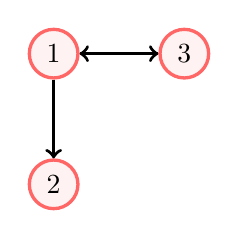
\begin{tikzpicture}[
	nstyle/.style={circle, fill=red!5, draw=red!60, very thick, 
	minimum size=5mm,}
	]
	\node[nstyle] (1) {$1$};
	\node[nstyle] (2) [below=of 1] {$2$};
	\node[nstyle] (3) [right=of 1] {$3$};
	
	\draw[->,very thick] (1.south) to (2.north);
	\draw[<-,very thick] (3.west) to (1.east);
	\draw[->,very thick] (3.west) to (1.east);
	\end{tikzpicture}\end{center}
	Is not possible. In fact such an ordering exists if and only if the
	graph we are trying to sort is a DAG.
	
	\newpage
	\noindent For example here is a DAG:
	\begin{center}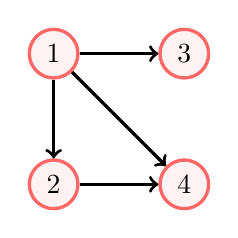
\begin{tikzpicture}[
	nstyle/.style={circle, fill=red!5, draw=red!60, very thick, 
	minimum size=5mm,}
	]
	\node[nstyle] (1) {$1$};
	\node[nstyle] (2) [below=of 1] {$2$};
	\node[nstyle] (3) [right=of 1] {$3$};
	\node[nstyle] (4) [below=of 3] {$4$};
	
	\draw[->,very thick] (1.south) to (2.north);
	\draw[->,very thick] (1.east) to (3.west);
	\draw[->,very thick] (1.south east) to (4.north west);
	\draw[->,very thick] (2.east) to (4.west);
	\end{tikzpicture}\end{center}
	A possible topological sorting is $(1,2,3,4)$ because we get:
	\begin{center}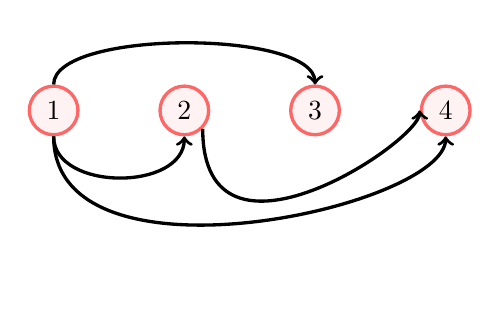
\begin{tikzpicture}[
	nstyle/.style={circle, fill=red!5, draw=red!60, very thick, 
	minimum size=5mm,}
	]
	\node[nstyle] (1) {$1$};
	\node[nstyle] (2) [right=of 1] {$2$};
	\node[nstyle] (3) [right=of 2] {$3$};
	\node[nstyle] (4) [right=of 3] {$4$};
	
	\draw[->,very thick] 
	(1.south) .. controls +(down:7mm) and +(down:7mm) .. (2.south);
	\draw[->,very thick] 
	(1.north) .. controls +(up:7mm) and +(up:7mm) .. (3.north);
	\draw[->,very thick] 
	(1.south) .. controls +(down:20mm) and +(down:9mm) .. (4.south);
	\draw[->,very thick] 
	(2.south east) .. controls +(0,-2) and +(down:4mm) .. (4.west);
	\end{tikzpicture}\end{center}
	
	
	
	\begin{algorithm}
	\caption{Kahn's Algorithm for Topological Sorting}
	\KwIn{Directed Acyclic Graph (DAG) $G=(V, E)$}
	\KwOut{Topologically sorted order of vertices}
	Compute in-degrees of all vertices\;
	Initialize queue $Q$ with all vertices of in-degree 0;
	\tcp{Also known as sources}\
	Initialize empty list $L$\;
	\While{$Q$ is not empty}{
		Dequeue a vertex $v$ from $Q$\;
		Append $v$ to $L$\;
		\For{each neighbor $u$ of $v$}{
		    Decrement in-degree of $u$\;
		    \If{in-degree of $u$ becomes 0}{
		        Enqueue $u$ to $Q$\;
		    }
		}
	}
	\eIf{$L$ contains all vertices}{
		\Return $L$\;
	}{
		\textbf{Error:} Graph has at least one cycle\;
	}
	\end{algorithm}
	
	

\end{document}